\documentclass[paper=a4,
               fontsize=11pt,
               bibliography=totoc,
               listof=nochaptergap,
               listof=notoc,
               numbers=noendperiod,
               parskip=half,
               footnotes=multiple,
               toc=numberline,
               captions=tableheading,
               DIV=10,
               %DIV=calc,
               %BCOR=5mm,
              ]{scrreprt}

\usepackage{scrhack}
\setcounter{tocdepth}{3}
\setcounter{secnumdepth}{3}

\deffootnote[1.5em]{1.5em}{1em}{\thefootnotemark. }
\addtokomafont{captionlabel}{\bfseries}
\setcapwidth[c]{.95\linewidth}

\usepackage{caption}
\usepackage{subcaption}
\DeclareCaptionLabelFormat{continued}{#1~#2 (\emph{Cont.})}
\captionsetup[ContinuedFloat]{labelformat=continued}

\usepackage[utf8]{inputenc}
\usepackage[T1]{fontenc}
\usepackage[english]{babel}
\usepackage{etoolbox}
\usepackage{xifthen}

%\usepackage[margin=3.5cm,bottom=4cm]{geometry}

\usepackage{amssymb}
\usepackage{libertine}
\usepackage[scaled=0.79]{beramono}
\usepackage{textcomp}
\usepackage[onehalfspacing]{setspace}
\usepackage{pdflscape}
\AfterTOCHead{\singlespacing}
\recalctypearea
\usepackage{xspace}

\usepackage[svgnames]{xcolor}
\definecolor{comment}{HTML}{236E25}
\definecolor{keyword}{HTML}{881280}
\definecolor{ndkeyword}{HTML}{994500}
\definecolor{string}{HTML}{1A1AA6}

\usepackage{graphicx}

\usepackage{tabularx}
\newcolumntype{b}{>{\bfseries}c}
\usepackage{booktabs}
\usepackage{multirow}
\usepackage{multicol}

\usepackage{enumitem}
\setlist{nolistsep}

\usepackage{tikz}
\usetikzlibrary{decorations.markings}
\usetikzlibrary{patterns}

\usepackage[hyphens]{url}
\urlstyle{same}
\renewcommand{\UrlBreaks}{%
  \do\a\do\b\do\c\do\d\do\e\do\f\do\g\do\h\do\i\do\j\do\k\do\l\do\m\do\n\do\o%
  \do\p\do\q\do\r\do\u\do\v\do\w\do\x\do\y\do\z\do\A\do\B\do\C\do\D\do\E\do\F%
  \do\G\do\H\do\I\do\J\do\K\do\L\do\M\do\N\do\O\do\P\do\Q\do\R\do\U\do\V\do\W%
  \do\X\do\Y\do\Z\do\_\do\/\do\-}

\usepackage[unicode]{hyperref}
\hypersetup{
  breaklinks,
  hidelinks,
  colorlinks=true,
  urlcolor=black,
  linkcolor=black,
  citecolor=black,
  pdfauthor={Christian Autermann},
  pdfsubject={Master-Thesis},
  pdftitle={Streaming Web-Services for Calculating Live Hydrological Derivatives}
}
\usepackage[capitalise,noabbrev,nameinlink]{cleveref}
\crefname{lstlisting}{listing}{listings}
\Crefname{lstlisting}{Listing}{Listings}

\usepackage[authoryear,round,comma,compress]{natbib}
\bibliographystyle{plainnat}

\usepackage{acronym}
\acrodef{WPS}{Web Processing Service}
\acrodef{OGC}{Open Geospatial Consortium}
\acrodef{DAG}{Directed Acyclic Graph}
\acrodef{BFS}{Breadth-first search}
\acrodef{CRS}{coordinate reference system}
\acrodef{XML}{Extensible Markup Language}
\acrodef{WSA}{Web Services Addressing}
\acrodef{OWS}{OGC Web Services Common}
\acrodef{CSW}{Catalogue Service for the Web}
\acrodef{WCS}{Web Coverage Service}
\acrodef{WMS}{Web Map Service}
\acrodef{SOS}{Sensor Observation Service}
\acrodef{GPGPU}{general-purpose computing on graphics processing units}
\acrodef{KVP}{key value pair}
\acrodef{GUID}{Globally Unique Identifier}
\acrodef{JVM}{Java Virtual Machine}
\acrodef{RMI}{Remote Method Invocation}
\acrodef{API}{Application Programming Interface}
\acrodef{GDP}{Geo Data Portal}
\acrodef{TSV}{Tab Seperated Values}
\acrodef{CSV}{Comma Seperated Values}
\acrodef{GML}{Geography Markup Language}
\acrodef{CORS}{Cross-Origin Resource Sharing}
\acrodef{HTTP}{Hypertext Transfer Protocol}

\newcommand{\acrocitep}[2]{\acl{#1} \citep[\acs{#1},][]{#2}}

\usepackage[squaren,binary,textstyle]{SIunits}

\usepackage{scrpage2}
\clearscrheadfoot
\cfoot[\pagemark]{\pagemark}

\usepackage[final]{listings}
\makeatletter
\def\addToLiterate#1{\edef\lst@literate{\unexpanded\expandafter{\lst@literate}\unexpanded{#1}}}
\lst@Key{moreliterate}{}{\addToLiterate{#1}}
\makeatother

\lstset{%
  numberstyle=\ttfamily\small,
  basicstyle=\ttfamily\small\mdseries\singlespacing,
  backgroundcolor=\color{white},
  commentstyle=\color{comment},
  stringstyle=\color{string},
  identifierstyle=\color{black},
  keywordstyle=\color{keyword}\bfseries,
  ndkeywordstyle=\color{ndkeyword},
  lineskip={-2.5pt}
}
\lstset{%
  %columns=fullflexible,
  breakatwhitespace=false,
  breaklines=true,
  showstringspaces=false,
  tabsize=2,
  captionpos=t,
  frame=L,
  frameround=ffff,
  numbers=left,
  stepnumber=5,
  numberfirstline=false,
  firstnumber=1,
  xleftmargin=2\bigskipamount,
  framexleftmargin=0pt,
  xrightmargin=2\bigskipamount,
  framexrightmargin=2\bigskipamount,
  aboveskip=\bigskipamount,
  belowskip=\bigskipamount,
}

\lstset{moreliterate=
  {á}{{\'a}}1 {é}{{\'e}}1 {í}{{\'i}}1 {ó}{{\'o}}1 {ú}{{\'u}}1
  {Á}{{\'A}}1 {É}{{\'E}}1 {Í}{{\'I}}1 {Ó}{{\'O}}1 {Ú}{{\'U}}1
  {à}{{\`a}}1 {è}{{\'e}}1 {ì}{{\`i}}1 {ò}{{\`o}}1 {ù}{{\`u}}1
  {À}{{\`A}}1 {È}{{\'E}}1 {Ì}{{\`I}}1 {Ò}{{\`O}}1 {Ù}{{\`U}}1
  {ä}{{\"a}}1 {ë}{{\"e}}1 {ï}{{\"i}}1 {ö}{{\"o}}1 {ü}{{\"u}}1
  {Ä}{{\"A}}1 {Ë}{{\"E}}1 {Ï}{{\"I}}1 {Ö}{{\"O}}1 {Ü}{{\"U}}1
  {â}{{\^a}}1 {ê}{{\^e}}1 {î}{{\^i}}1 {ô}{{\^o}}1 {û}{{\^u}}1
  {Â}{{\^A}}1 {Ê}{{\^E}}1 {Î}{{\^I}}1 {Ô}{{\^O}}1 {Û}{{\^U}}1
  {œ}{{\oe}}1 {Œ}{{\OE}}1 {æ}{{\ae}}1 {Æ}{{\AE}}1 {ß}{{\ss}}1
  {ç}{{\c c}}1 {Ç}{{\c C}}1 {ø}{{\o}}1 {å}{{\r a}}1 {Å}{{\r A}}1
  {€}{{\EUR}}1 {£}{{\pounds}}1 {°}{{\textdegree}}1
  {µ}{{$\mathrm{\mu}$}}1 {μ}{{$\mathrm{\mu}$}}1
  {±}{{$\pm$}}1 {σ}{{$\mathrm{\sigma}$}}1
  {⋅}{{$\cdot$}}1 {‘}{`}1 {’}{'}1
}

\lstdefinelanguage{yaml}{
  keywords={true, false, null, y, n},
  sensitive=false,
  comment=[l]{\#},
  morecomment=[s]{/*}{*/},
  moredelim=[l][\color{ndkeyword}]{\&},
  moredelim=[l][\color{ndkeyword}]{*},
  moredelim=**[il][\textcolor{ndkeyword}{:}]{:},
  morestring=[b]',
  morestring=[b]",
  moreliterate = {---}{{\textcolor{ndkeyword}{-{-}-}}}3
                 {...}{{\textcolor{ndkeyword}{...}}}3
                 {>}{{\textcolor{ndkeyword}\textgreater}}1
                 {|}{{\textcolor{ndkeyword}\textbar}}1
                 {\ -\ }{{\textcolor{ndkeyword}{\ -\ }}}3
}

\lstdefinelanguage{JavaScript}{
  morekeywords={
    break, case, catch, continue, debugger, default, delete, do, else, finally, for, function, if, in, instanceof, new,
    return, switch, this, throw, try, typeof, var, while, with, null, throw, this
  },
  morendkeywords={
    Object, Array, Boolean, Date, window, Number, String, Math, XMLHttpRequest, document, prototype, undefined, Infinity,
    WebSocket, NaN, import, export, this, console, Error
  },
  sensitive,
  comment=[l]{//},
  morecomment=[s]{/*}{*/},
  morestring=[b]',
  morestring=[b]",
}
\lstdefinelanguage{XML}{
  morestring=[b]",
  morecomment=[s]{<?}{?>},
  morecomment=[s]{<!--}{-->},
  morecomment=[s]{&}{;},
  alsoletter={:},
  morekeywords={
    ComplexData, ComplexOutput, DataInputs, Default, Encoding, Format, hello, Input, LiteralData, LiteralOutput, MimeType,
    Output, ows:Abstract, ows:AllowedValues, ows:AnyValue, ows:DataType, ows:Exception, ows:ExceptionText, ows:Identifier,
    ows:LowerCorner, ows:Title, ows:UOM, ows:UpperCorner, ows:Value, ProcessDescription, ProcessOutputs, soap:Body,
    soap:Envelope, soap:Header, stream:DescribeMessage, stream:DescriptionMessage, stream:ErrorMessage, stream:InputMessage,
    stream:Inputs, stream:Output, stream:OutputMessage, stream:OutputRequestMessage, stream:Outputs, stream:ProcessID,
    stream:Reference, stream:ReferenceInput, stream:StaticInputs, stream:StopMessage, stream:StreamingInput,
    stream:StreamingProcessDescription, Supported, UOMs, wps:BoundingBoxData, wps:ComplexData, wps:Data, wps:DataInputs,
    wps:Execute, wps:ExecuteResponse, wps:Input, wps:LiteralData, wps:Output, wps:Process, wps:ProcessDescriptions,
    wps:ProcessOutputs, wps:ProcessSucceeded, wps:Reference, wps:Status, wsa:Action, wsa:Address, wsa:FaultTo, wsa:From,
    wsa:MessageID, wsa:RelatesTo, wsa:ReplyTo, wsa:To,
  },
  morendkeywords={
    creationTime, crs, dataType, dimensions, encoding, exceptionCode, finalResult, includeInputs, intermediateResults,
    maxOccurs, method, mimeType, minOccurs, ows:reference, RelationshipType, service, serviceInstance, statusSupported,
    storeSupported, version, wps:processVersion, xlink:href, xml:lang, xmlns:ows, xmlns:soap, xmlns:stream, xmlns:wps,
    xmlns:wsa, xmlns:xlink, schema
  }
}

\newcommand{\fu}[1]{\footnote{\url{#1}}}
\newcommand{\mail}[1]{\href{mailto:#1}{#1}}
\newcommand{\texttag}[2]{{\ttfamily\textless#1:#2\textgreater}}

\newcommand{\sign}[1]{{%
  \leavevmode\unskip\nobreak\hfil\penalty50\hskip2em\hbox{}\nobreak\hfil%
  \textup{\small--- #1}\parfillskip=0pt\finalhyphendemerits=0\endgraf%
}}

\newsavebox\signedbox
\newenvironment{xquote}[1][]
  {\savebox\signedbox{#1}\quote\itshape}
  {\ifthenelse{\isempty{\usebox\signedbox}}{\sign{\usebox\signedbox}}\endquote}

\newcommand{\ftn}{52\textdegree{}North\xspace}
\newcommand{\la}{LakeAnalyzer\xspace}
\renewcommand{\lstlistlistingname}{List of Listings}
\renewenvironment{bold}{\bfseries}{}
\newenvironment{italic}{\itshape}{}
\newenvironment{smallcaps}{\scshape}{}
\newenvironment{slanted}{\slshape}{}
\newenvironment{sansserif}{\sffamily}{}
\newenvironment{serif}{\rmfamily}{}
\newenvironment{fixedwidth}{\ttfamily}{}
\newenvironment{listings}{\pagestyle{scrplain}\pagenumbering{roman}}{\clearpage}
\newenvironment{content}{\pagestyle{scrheadings}\pagenumbering{arabic}}{\bibliography{\jobname}\clearpage}
\AtBeginEnvironment{appendix}{
    \pagestyle{scrplain}
    \pagenumbering{roman}
    \KOMAoptions{chapterprefix}
    \lstset{%
      numberstyle=\ttfamily\footnotesize,
      basicstyle=\ttfamily\footnotesize\mdseries\singlespacing,
      lineskip={-2pt}
    }
  }
\AtEndEnvironment{appendix}{\clearpage}
\AtEndEnvironment{listings}{\clearpage}
\AtEndEnvironment{contents}{\clearpage}

\begin{document}
  \begin{titlepage}
    \begin{spacing}{1}
      \onehalfspacing
      \begin{center}
        \begin{large}
          \textbf{Master Thesis}\\
          \vspace{1cm}
          \begin{huge}
            \begin{bold}
              \begin{sansserif}
                Streaming Web-Services for Calculating Live Hydrological Derivatives\\
              \end{sansserif}
            \end{bold}
          \end{huge}
          \vspace*{1cm}
          \begin{italic}
            By\\
          \end{italic}
          \begin{bold}
            Christian Autermann\\
          \end{bold}
          \mail{autermann@uni-muenster.de}\\
          Matriculation Number: 347760\\
          \vspace{1cm}
          \begin{italic}
            Submitted to the\\
          \end{italic}
          Institute for Geoinformatics\\
          University of Münster\\
          \vspace{1cm}
          \begin{italic}
            In Partial Fulfillment of the Requirements for the Degree\\
          \end{italic}
          Master of Science in Geoinformatics\\
          \vspace{1cm}
          \begin{bold}
            \today\\
          \end{bold}
          \vspace*{\fill}
          \begin{bold}
            Supervisors:
          \end{bold}
          \\\vspace{.5cm}
          \begin{tabular}{cc}
            \textbf{Prof. Dr. Edzer Pebesma}     & \textbf{Jordan S. Read, PhD} \\
            %\mail{edzer.pebesma@uni-muenster.de} & \mail{jread@usgs.gov}\\
            Institute for Geoinformatics         & Center for Integrated Data Analysis\\
            University of Münster                & United States Geological Survey\\
          \end{tabular}
        \end{large}
      \end{center}
    \end{spacing}
  \end{titlepage}
  \begin{listings}
    \begingroup
      \renewcommand{\clearpage}{}
      \tableofcontents
      \listoftables
      \listoffigures
      \lstlistoflistings
    \endgroup
  \end{listings}

  \begin{content}
    %!TEX root = thesis.tex
\section{Introduction}
	\section{Lake-Analyzer}
	\section{Foundtations}
		\subsection{Limniography}
		\subsection{Web Processing Service}
		\subsection{Streaming}
			\subsubsection{WebSockets}
		\subsection{Matlab}
		\subsection{WPS4R}
		\subsection{Previous approaches}
	\section{Matlab WPS}


		\newcommand{\listing}

		\subsection{Configuration}
		\includecode[Matlab]
			{matlab-add-function.m}
			{\label{lst:matlab:example:fun}Matlab example function.}
		\includecode[YAML,morekeywords={function,connection,identifier,version,inputs,outputs,type}]
			{matlab-add-process-configuration.yaml}
			{\label{lst:matlab:example:yaml}Matlab process configuration describing the function in Listing \ref{lst:matlab:example:fun}.}
		\includecode[XML]
			{matlab-add-process-description.xml}
			{\label{lst:matlab:example:desc}Process description generated from the configuration in Listing \ref{lst:matlab:example:yaml}.}

		\subsection{Type Mapping}
		\begin{table}[!htb]
			\sffamily\centering
			\caption{\label{tab:matlab:typemapping}Type Mapping between Matlab and WPS Data}
			\begin{tabular}{@{}llcc@{}}
				\toprule
				&
				& \multicolumn{2}{b}{Matlab Type}\\
				\cmidrule(l){3-4}
				\multicolumn{1}{@{}b}{}
				& \multicolumn{1}{b}{Data}
				& \multicolumn{1}{b}{For single inputs}
				& \multicolumn{1}{b@{}}{For multiple inputs}\\
				\cmidrule(rl){2-2}
				\cmidrule(rl){3-3}
				\cmidrule(l){4-4}
				\textbf{Complex}      & \textit{any} & String  & Cell \\\midrule
				\textbf{Bounding Box} & -            & -       & -    \\\midrule
				\textbf{Literal}      & xs:int       & Numeric & Array\\
								      & xs:boolean   & Numeric & Array\\
								      & xs:dateTime  & Numeric & Array\\
								      & xs:double    & Numeric & Array\\
								      & xs:float     & Numeric & Array\\
								      & xs:byte      & Numeric & Array\\
								      & xs:short     & Numeric & Array\\
								      & xs:int       & Numeric & Array\\
								      & xs:long      & Numeric & Array\\
								      & xs:string    & String  & Cell \\
								      & xs:anyURI    & String  & Cell \\
				\bottomrule
			\end{tabular}
		\end{table}
		\subsection{Pooling}
		\subsection{License Issues}
		\subsection{Implementation}
		\begin{figure}[!htb]
			\centering
			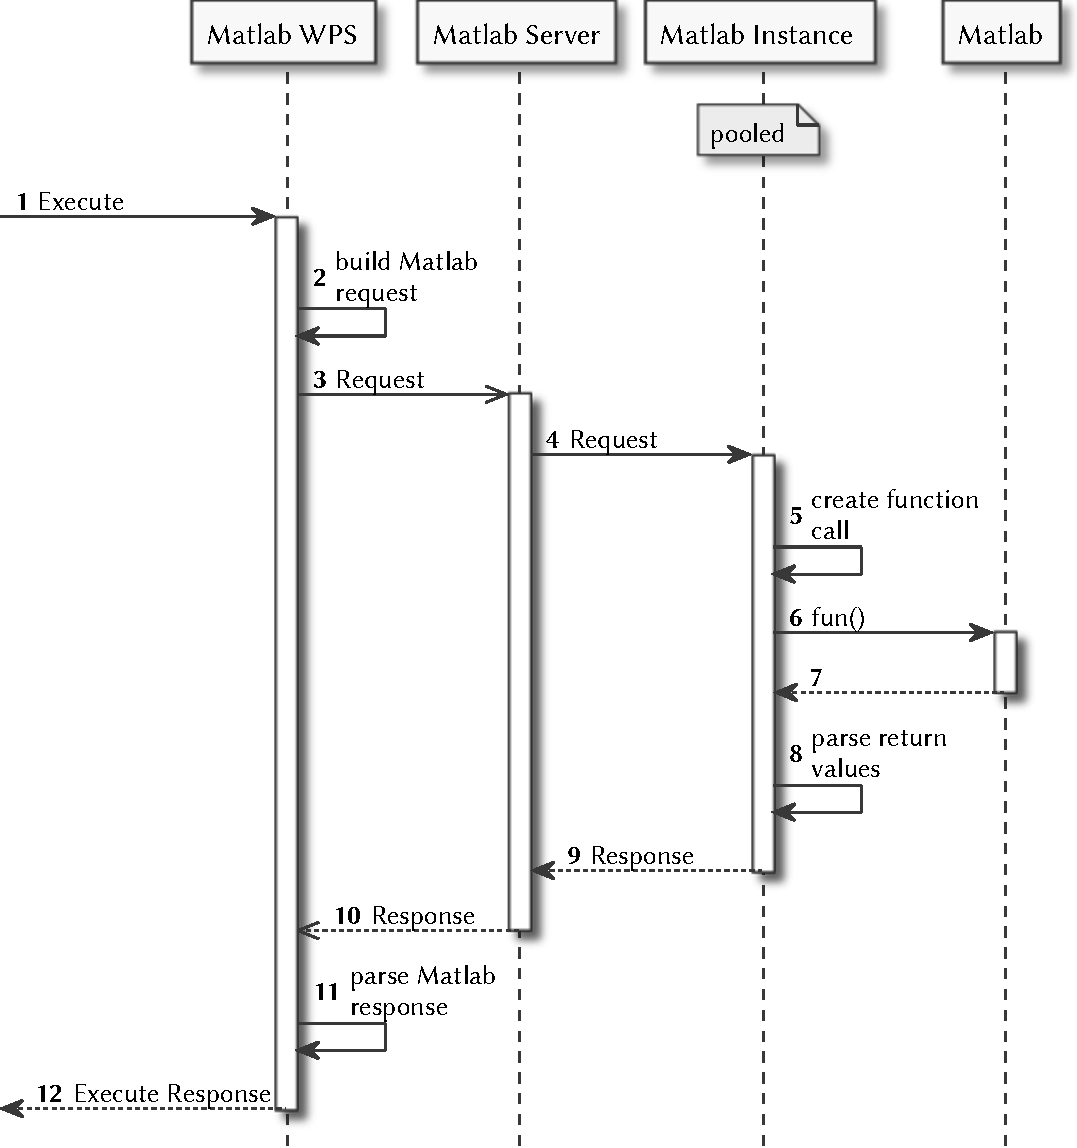
\includegraphics[width=.8125\textwidth]{figures/sequence-diagramm-mwps.pdf}
			\caption{\label{fig:sd:mwps} Sequence diagram of the Matlab WPS.} %182x194
		\end{figure}
		\subsection{Lake-Analyzer WPS}
	\section{Streaming WPS}
		\subsection{Input Types}
		\subsection{Dependencies}
		\begin{figure}[!htb]
			\centering
			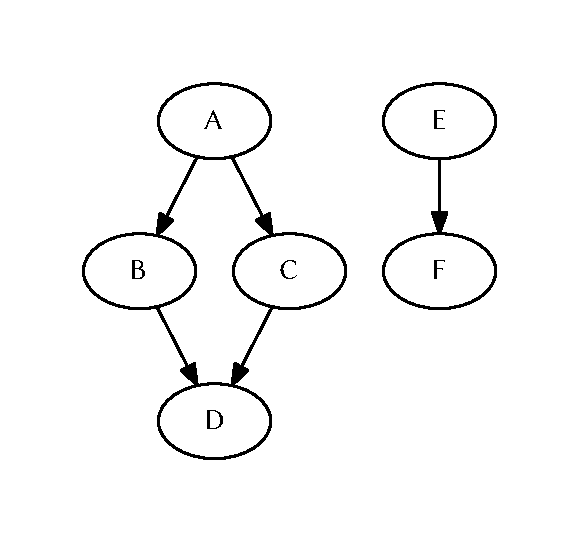
\includegraphics[width=.4474\textwidth]{figures/unordered-graph.pdf} % 98x92
			\caption{\label{fig:graph:unordered} Example for a dependency graph.}
		\end{figure}
		\begin{figure}[!htb]
			\centering
			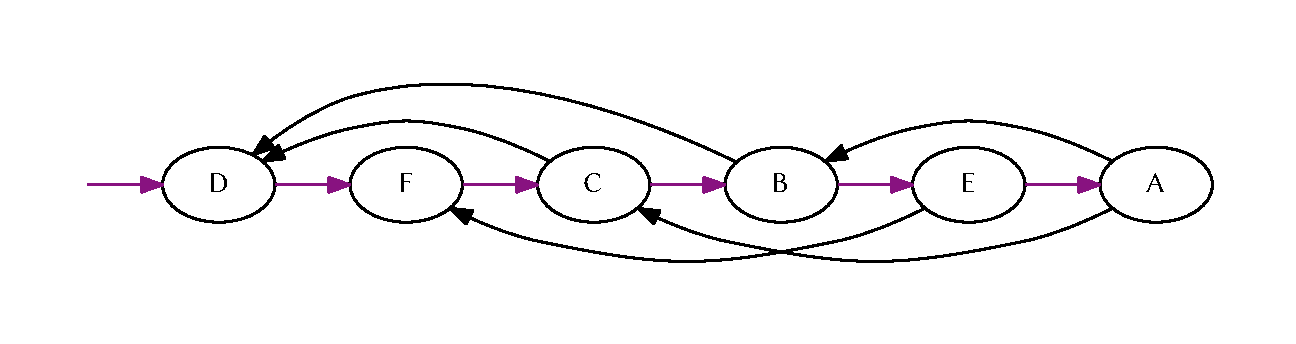
\includegraphics[width=1\textwidth]{figures/ordered-graph.pdf} % 219x58
			\caption{\label{fig:graph:ordered} Topological ordering for of the dependency graph in Figure \ref{fig:graph:unordered}.}
		\end{figure}

		\subsection{Protocoll}
		\subsection{Implementation}
		\begin{figure}[!htb]
			\centering
			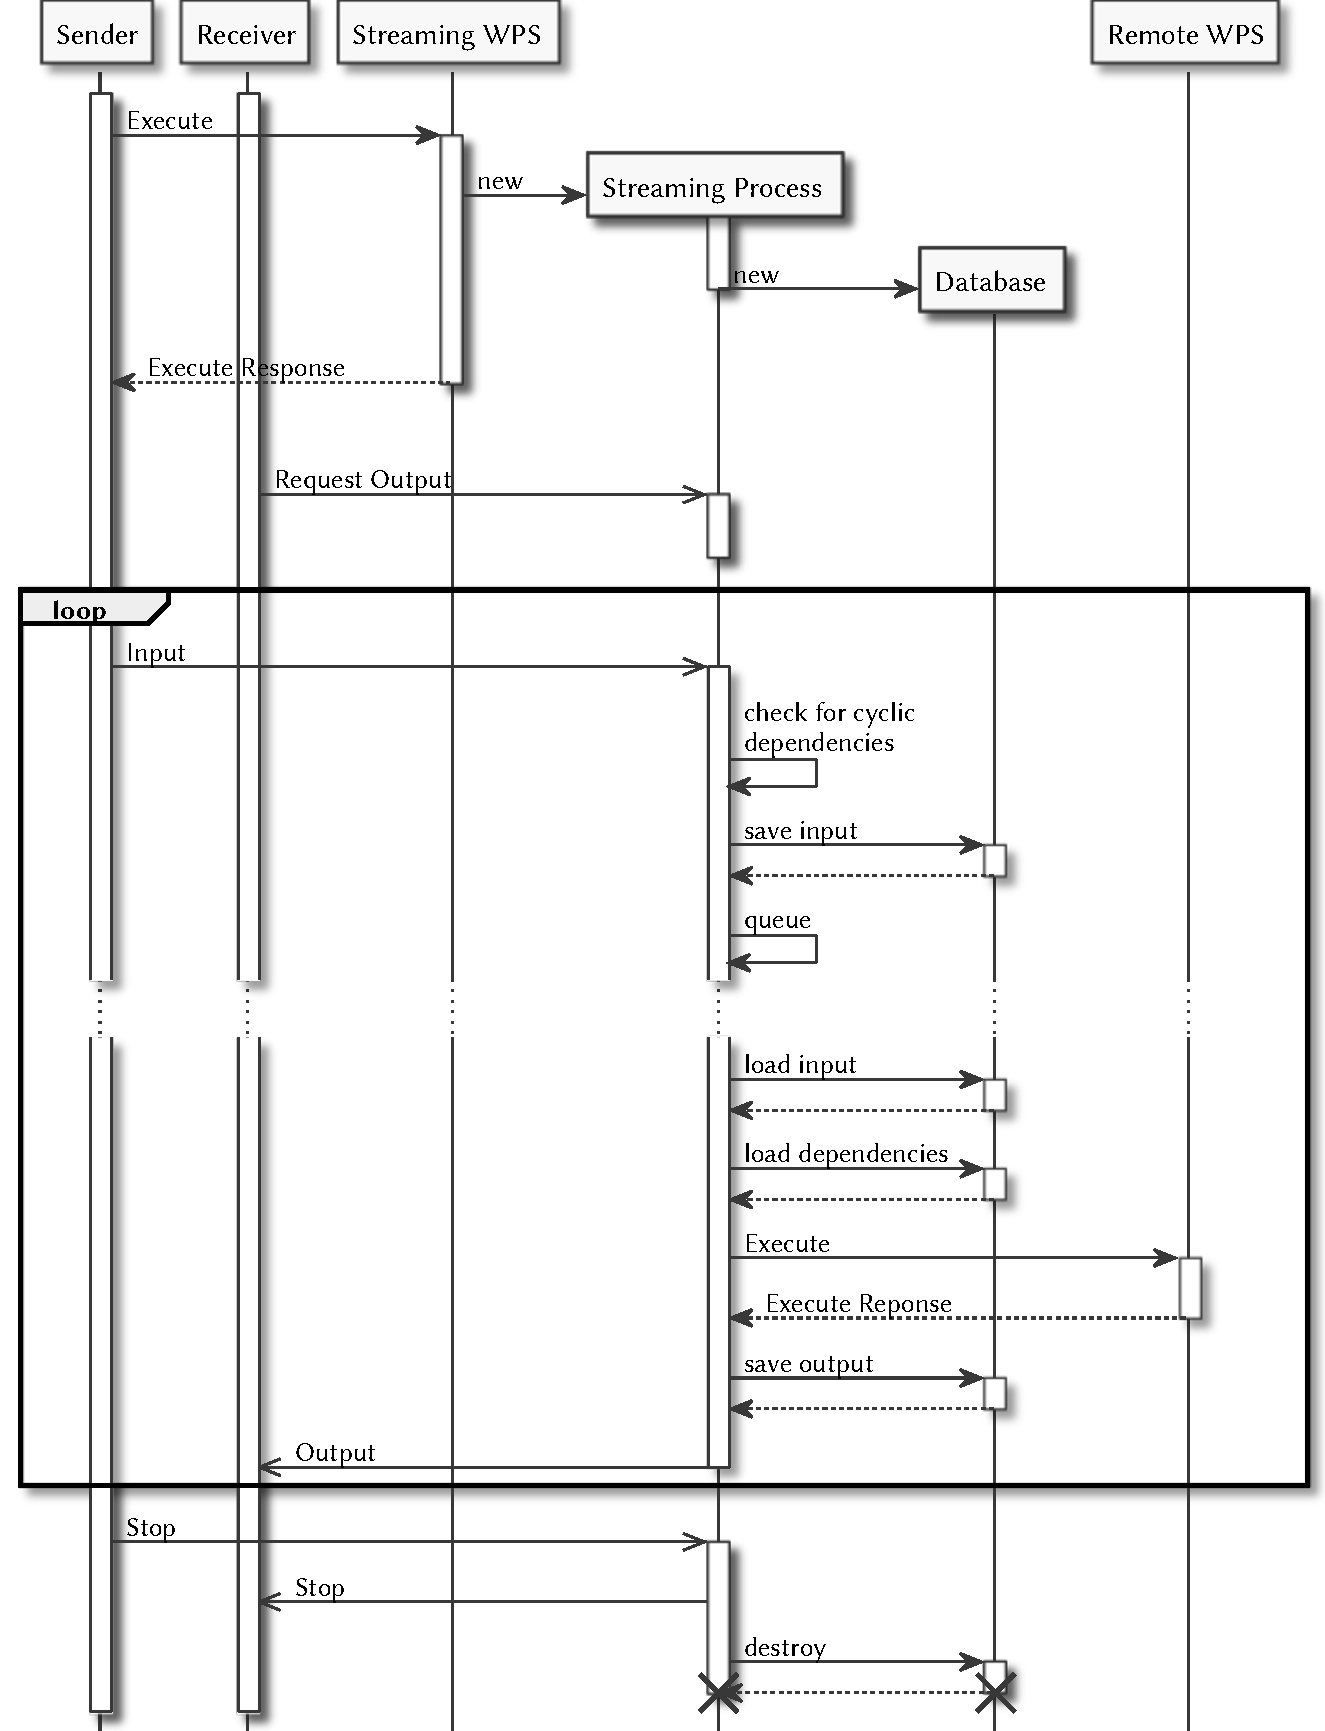
\includegraphics[width=1\textwidth]{figures/sequence-diagramm-swps.pdf}
			% 224x293
			\caption{\label{fig:sd:swps} Sequence diagram of the Streaming WPS.}
		\end{figure}
		\subsection{Client Implementation}
		\subsection{Streaming Lake-Analyzer WPS}
	\section{Future Work}
	\section{Conclusion}
  \end{content}

  \begin{appendix}
    \chapter{Lake Analyzer Process Wrapper Function}
      \label{appendix:lakeanalyzer:wrapper}
      \lstinputlisting[nolol,language=MATLAB, morekeywords={struct},morendkeywords={Run_LA_WPS,LA},moreliterate = {...}{{\textcolor{ndkeyword}{...}}}3]{listings/lake-analyzer-wps-wrapper.m}

    \chapter{Lake Analyzer Process Configuration}
      \label{appendix:lakeanalyzer:configuration}
      \lstinputlisting[nolol,language=YAML,label={lst:matlab:lakeanalyzer:yaml},morekeywords={function,connection,identifier,version,inputs,outputs,type,host,port,title,abstract,mimeType,encoding,schema,unit,minOccurs,maxOccurs,values}]{listings/lake-analyzer-wps-configuration.yaml}

    \chapter{Lake Analyzer Process Description}
      \label{appendix:lakeanalyzer:description}
      See \cref{sec:xmlnamespaces} for omitted XML namespaces.
      \lstinputlisting[nolol,language=XML]{listings/lake-analyzer-wps-process-description.xml}

    \chapter{Source Code}
      All source code, including prototypical implementations of the described Streaming WPS and MATLAB WPS, is freely available under an open source license:
      \begin{center}
        \begin{small}
          \begin{tabularx}{\linewidth}{@{}lX@{}}
          \toprule
            \textbf{Streaming WPS}
            & Extension for the \ftn WPS to allow streaming of input and output parameters over WebSockets.\\
            & GNU General Public License Version 3\\
            & \url{https://github.com/autermann/streaming-wps} \\
            \cmidrule(r){1-1}
            \cmidrule(l){2-2}

            \textbf{MATLAB WPS}
            & Extension for the \ftn WPS to offer MATLAB functions and scripts as OGC Web Processing Service algorithms.\\
            & GNU General Public License Version 2\\
            & \url{https://github.com/autermann/matlab-wps}\\
            \cmidrule(r){1-1}
            \cmidrule(l){2-2}

            \textbf{streaming-wps-js}
            & Streaming WPS JavaScript Bindings\\
            & Apache License Version 2.0\\
            & \url{https://github.com/autermann/streaming-wps-js}\\
            \cmidrule(r){1-1}
            \cmidrule(l){2-2}

            \textbf{WPS Commons}
            & \ftn WPS convenience classes and bootstrapping code.\\
            & GNU General Public License Version 2\\
            & \url{https://github.com/autermann/wps-commons}\\
            \cmidrule(r){1-1}
            \cmidrule(l){2-2}

            \textbf{MATLAB Connector}
            & MATLAB function execution on (pooled) remote MATLAB instances.\\
            & GNU General Public License Version 3\\
            & \url{https://github.com/autermann/matlab-connector}\\
            \cmidrule(r){1-1}
            \cmidrule(l){2-2}

            \textbf{LakeAnalyzer}
            & MATLAB source code for Lake Analyzer\\
            & GNU General Public License Version 2\\
            & \url{https://github.com/autermann/Lake-Analyzer}\\
            \cmidrule(r){1-1}
            \cmidrule(l){2-2}

            \textbf{YAML API}
            & A Jackson-like API to read and create YAML nodes (based on SnakeYAML).\\
            & Apache License Version 2.0\\
            & \url{https://github.com/autermann/yaml}\\
            \bottomrule
          \end{tabularx}
        \end{small}
      \end{center}


    \chapter{XML Namespaces}\label{sec:xmlnamespaces}
      For clarity XML name spaces are omitted in XML Listings. Their respective value can be found in the following table:
      \begin{center}
        \begin{small}
          \begin{tabular}{@{}ll@{}}
            \toprule
            \textbf{Prefix} & \textbf{Namespace} \\
            \midrule
            xlink  & \url{http://www.w3.org/1999/xlink}\\
            xml    & \url{http://www.w3.org/XML/1998/namespace}\\
            xs     & \url{http://www.w3.org/2001/XMLSchema}\\
            xsi    & \url{http://www.w3.org/2001/XMLSchema-instance}\\
            %\addlinespace
            soap   & \url{http://www.w3.org/2003/05/soap-envelope}\\
            wsa    & \url{http://www.w3.org/2005/08/addressing}\\
            %\addlinespace
            ows    & \url{http://www.opengis.net/ows/1.1}\\
            wps    & \url{http://www.opengis.net/wps/1.0.0}\\
            %\addlinespace
            stream & \url{https://github.com/autermann/streaming-wps} \\
            \bottomrule
          \end{tabular}
        \end{small}
      \end{center}
  \end{appendix}

  \pagenumbering{gobble}
  \chapter*{Plagiarism Statement}
  Hiermit versichere ich, dass die vorliegende Arbeit über \emph{Streaming Web-Services for Calculating Live Hydrological Derivatives} selbstständig verfasst worden ist, dass keine anderen Quellen und Hilfsmittel als die angegebenen benutzt worden sind und dass die Stellen der Arbeit, die anderen Werken – auch elektronischen Medien – dem Wortlaut oder Sinn nach entnommen wurden, auf jeden Fall unter Angabe der Quelle als Entlehnung kenntlich gemacht worden sind.
  \begin{flushright}
    Münster, den 5. Mai 2014\hspace{.6cm}\rule{6cm}{.5pt}
  \end{flushright}
  \vspace{1cm}

  Ich erkläre mich mit einem Abgleich der Arbeit mit anderen Texten zwecks Auffindung von Übereinstimmungen sowie mit einer zu diesem Zweck vorzunehmenden Speicherung der Arbeit in eine Datenbank einverstanden.

  \begin{flushright}
    Münster, den 5. Mai 2014\hspace{.6cm}\rule{6cm}{.5pt}
  \end{flushright}

\end{document}